\documentclass[12pt]{article}
\usepackage{graphicx}
\usepackage{amsmath}
\usepackage{mathtools}
\usepackage{gensymb}

\newcommand{\mydet}[1]{\ensuremath{\begin{vmatrix}#1\end{vmatrix}}}
\providecommand{\brak}[1]{\ensuremath{\left(#1\right)}}
\providecommand{\norm}[1]{\left\lVert#1\right\rVert}
\newcommand{\solution}{\noindent \textbf{Solution: }}
\newcommand{\myvec}[1]{\ensuremath{\begin{pmatrix}#1\end{pmatrix}}}
\let\vec\mathbf

\begin{document}
\begin{center}
\textbf\large{CHAPTER-7 \\ COORDINATE GEOMETRY}
\end{center}
\section*{Excercise 7.2.9}

1. Find the coordinates of the point which divides the line segment joining $\vec(-2,2) \text{ and } \vec(2,8)$ into four equal parts
\\
\\
\solution\\		
Let the points $\vec{A}$,$\vec{B}$,$\vec{C}$ which divide the line into 4 equal parts\\
\\
Ratio of PAQ = 3:1\\
\\
Ratio of PBQ = 2:2\\
\\
Ratio of PCQ = 1:3\\
\\
coordinates and ratio are given as:
\begin{align}
\vec{P}=\myvec{-2\\2\\},
\vec{Q}=\myvec{2\\8\\},
\end{align}

\begin{enumerate}


\item Using section formula for n:
    
\begin{align}
n&=\frac{3}{1}\\
\vec{R}&=\frac{\vec{Q}+n\vec{P}}{1+n}\\
&=\frac{1}{1+\frac{3}{1}}  \myvec{\myvec{
2\\
8
}
  +
   \frac{3}{1}\myvec{
-2\\
2
}}\\
&= \frac{1}{\frac{4}{1}} \myvec{\myvec{
2\\
8
}
  +
\frac{1}{1}\myvec{
-6\\
6
}} \\
&=\frac{1}{4}
\myvec{
-4\\
14
}\\
&=\myvec{
-1\\
\\
\frac{7}{2}\\
}
\end{align}

\item Using section formula for n:
\begin{align}
n&=\frac{2}{2}\\
\vec{R}&=\frac{\vec{Q}+n\vec{P}}{1+n}\\
&=\frac{1}{1+\frac{2}{2}}  \myvec{\myvec{
2\\
8
}
  +
   \frac{2}{2}\myvec{
-2\\
2
}}\\
&= \frac{1}{\frac{4}{2}} \myvec{\myvec{
2\\
8
}
  +
\frac{1}{1}\myvec{
-2\\
2
}} \\
&=\frac{1}{2}
\myvec{
0\\
10
}\\
&=\myvec{
0\\
5
}
\end{align}

\item Using section formula for n:
\begin{align}
n&=\frac{1}{3}\\
\vec{R}&=\frac{\vec{Q}+n\vec{P}}{1+n}\\
&=\frac{1}{1+\frac{1}{3}}  \myvec{\myvec{
2\\
8
}
  +
   \frac{1}{3}\myvec{
-2\\
2
}}\\
&= \frac{1}{\frac{4}{3}} \myvec{\myvec{
2\\
8
}
  +
\myvec{
\frac{-2}{3}\\
\\
\frac{2}{3}\\
}} \\
&=\frac{3}{4}
\myvec{
\frac{4}{3}\\
\\
\frac{26}{3}\\
}\\
&=\myvec{
1\\
\\
\frac{13}{2}\\
}
\end{align}

\end{enumerate}
\begin{figure}[!h]
\begin{center}
   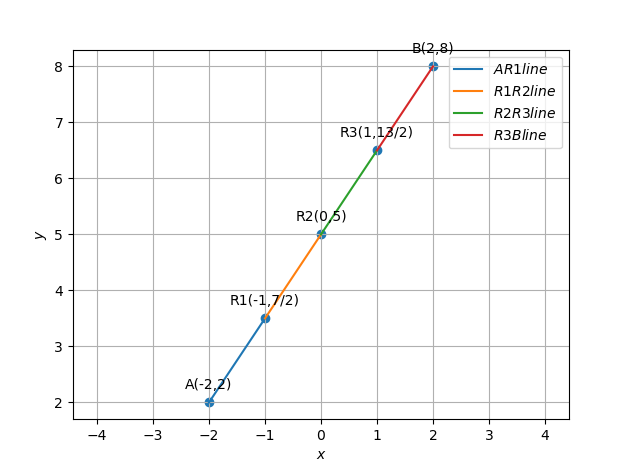
\includegraphics[width=\columnwidth]{./pics/7.2.9.png}
\end{center}
\caption{}
\label{fig:Fig}
\end{figure}


\end{document}